\subsection{Diseño}

Una vez compensado el sistema se procedió a diseñar el PCB. Para evitar problemas de interferencia electromagnética se tuvieron en cuenta las recomendaciones detalladas en la hoja de datos del regulador LM2576~\cite{LM2576_datasheet}. 

\begin{figure}[H]
    \centering
    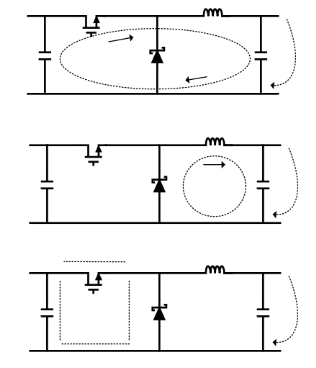
\includegraphics[width=0.9\textwidth]{img/PCB/Mallas.png}
    \caption{Mallas de la fuence \textit{buck}.}
    \label{fig:mallas}
\end{figure}

La mencionada hoja de datos provee la \autoref{fig:mallas} y destaca que la malla de la izquierda (la cual contiene al capacitor de entrada y a ambas llaves) es la más propensa a producir ruido ya que tiene elevados picos de corriente. De esta forma, si las pistas tuvieran una inductancia parásita elevada producirían altos picos de tensión en virtud de la ecuación del inductor 
\[
  v_L = L \frac{di_L}{dt}\,.
\]
Así, incluso con pequeños valores de $L$ se pueden producir picos elevados de $v_L$. Es entonces necesario reducir al máximo la inductancia parásita de las pistas, lo cual se consigue haciéndolas lo más anchas y cortas posibles y minimizando la superficie de la espira que forma la malla de entrada. 

\begin{figure}[H]
    \centering
    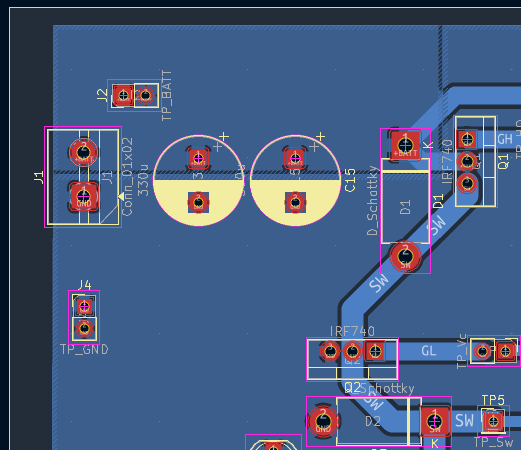
\includegraphics[width=0.9\textwidth]{img/PCB/Malla en el PCB.png}
    \caption{Malla de entrada en el PCB.}
    \label{fig:malla en el PCB}
\end{figure}

La \autoref{fig:malla en el PCB} muestra cómo se implementó la malla de entrada en el PCB, donde los capacitores electrolíticos forman el capacitor de entrada y los transistores $Q_1$ y $Q_2$ forman las llaves. 

\begin{figure}[H]
    \centering
    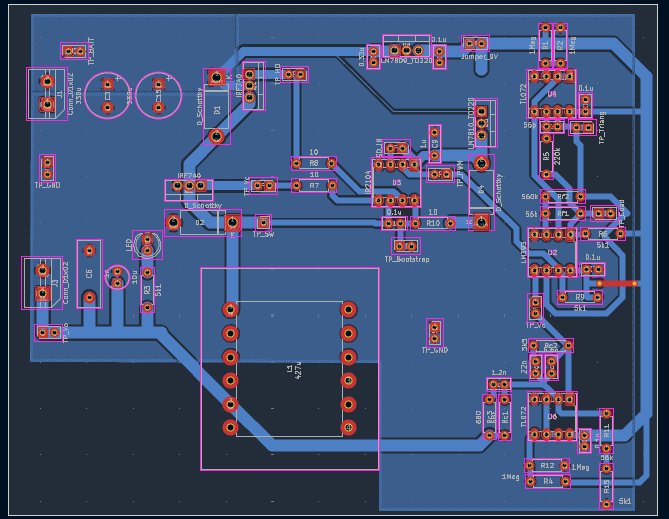
\includegraphics[width=0.9\textwidth]{img/PCB/PCB final.png}
    \caption{PCB final}
    \label{fig:PCB final}
\end{figure}

\begin{figure}[H]
    \centering
    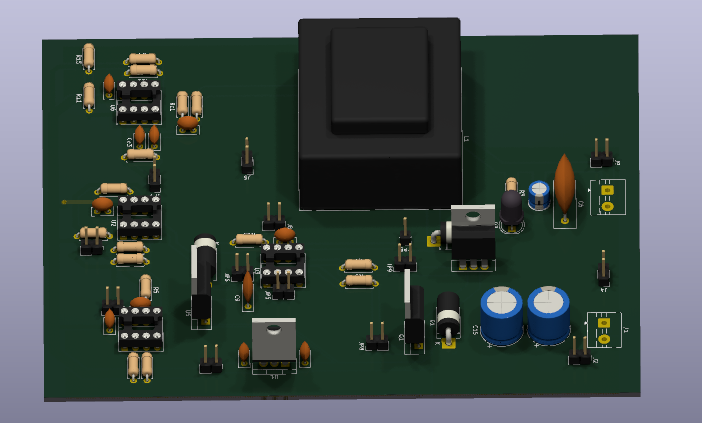
\includegraphics[width=0.9\textwidth]{img/PCB/PCB3D.png}
    \caption{Versión 3D del PCB}
    \label{fig:PCB3D}
\end{figure}

Las Figuras \ref{fig:PCB final} y \ref{fig:PCB3D} muestran el resultado final del diseño del PCB. 

\subsection{Implementación}

Dado que fue imposible delegar la manufactura del PCB por causas de fuerza mayor, la misma formó parte del desarrollo del \textit{checkpoint}.

\begin{figure}[H]
    \centering
    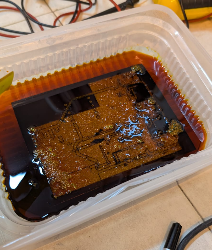
\includegraphics[width=0.9\textwidth]{img/PCB/PCB en acido.png}
    \caption{PCB en ácido.}
    \label{fig:PCB en ácido}
    
\end{figure}

La \autoref{fig:PCB en ácido} muestra el proceso de fabricación. Cabe mencionar que, si bien el mismo llevo más tiempo, también permitió un mayor grado de libertad en cuanto al tamaño de los agujeros y la correción de errores en el diseño original del PCB.

\begin{figure}[H]
    \centering
    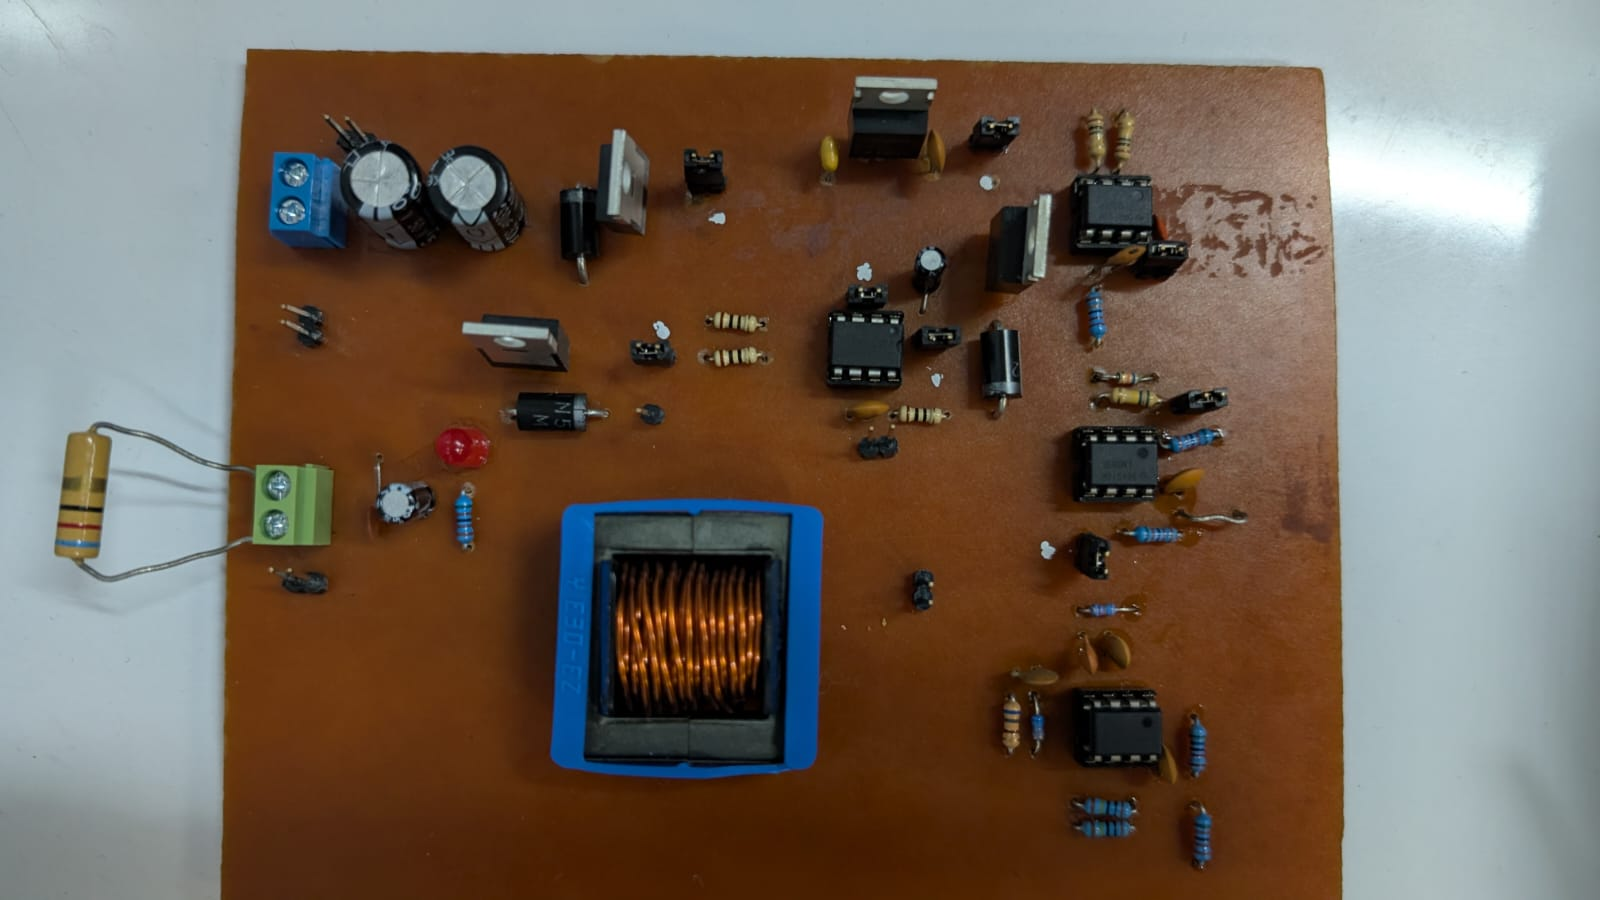
\includegraphics[width=0.9\textwidth]{img/PCB/pcb-final.jpeg}
    \caption{PCB final.}
    \label{fig:PCB_final}
    
\end{figure}

Por último, como se observa en la fig. \ref{fig:PCB_final} se puede apreciar la placa final terminada con los componentes soldados.
